\documentclass[a4paper,10pt]{article}
\usepackage[utf8]{inputenc}
%\usepackage[cm]{fullpage}
\usepackage[top=0.5in, bottom=1.5in, left=1.2in, right=1.2in]{geometry}
\usepackage{graphicx}

%\usepackage{showframe} %Just for Frame Testing.

%opening
\title{Master Thesis Proposal}
\author{Constantin Gaul - TU-Berlin, 315687}

\begin{document}

\maketitle

%\chapter{Master Thesis Proposal}
\section{Proposal Summary}
Based on a Cloud-Federation scenario, the scope of the Master Thesis will be to connect two or more Cloud Networks in order to form a horizontal federation, having the ability to route data from one network to the other, with a network encapsulation in place.\\
Today's Cloud Networks are commonly set up in a SDN fashion, enabling the possibility of changing routing paths in a flexible manner, mostly using OpenFlow. This gives a Cloud-Provider the possibility to use the virtualized network as a resource to be leased to his customers, as it is already the case in CPU virtualization, where customers could rent computing time on a specified "Compute-Unit".\\
As of that, a Cloud federation scenario does not only have to care about Cloud discovery and connection establishment, but more importantly it also needs to take care of the interconnection of the virtualized network environment in each federated Cloud. In order to form a federated virtual network, a federation management will be proposed that is able to route traffic through different virtual network scopes, enabling tenant networks to cross the border of one single physical network.

\begin{figure}[h!]
 \centering
 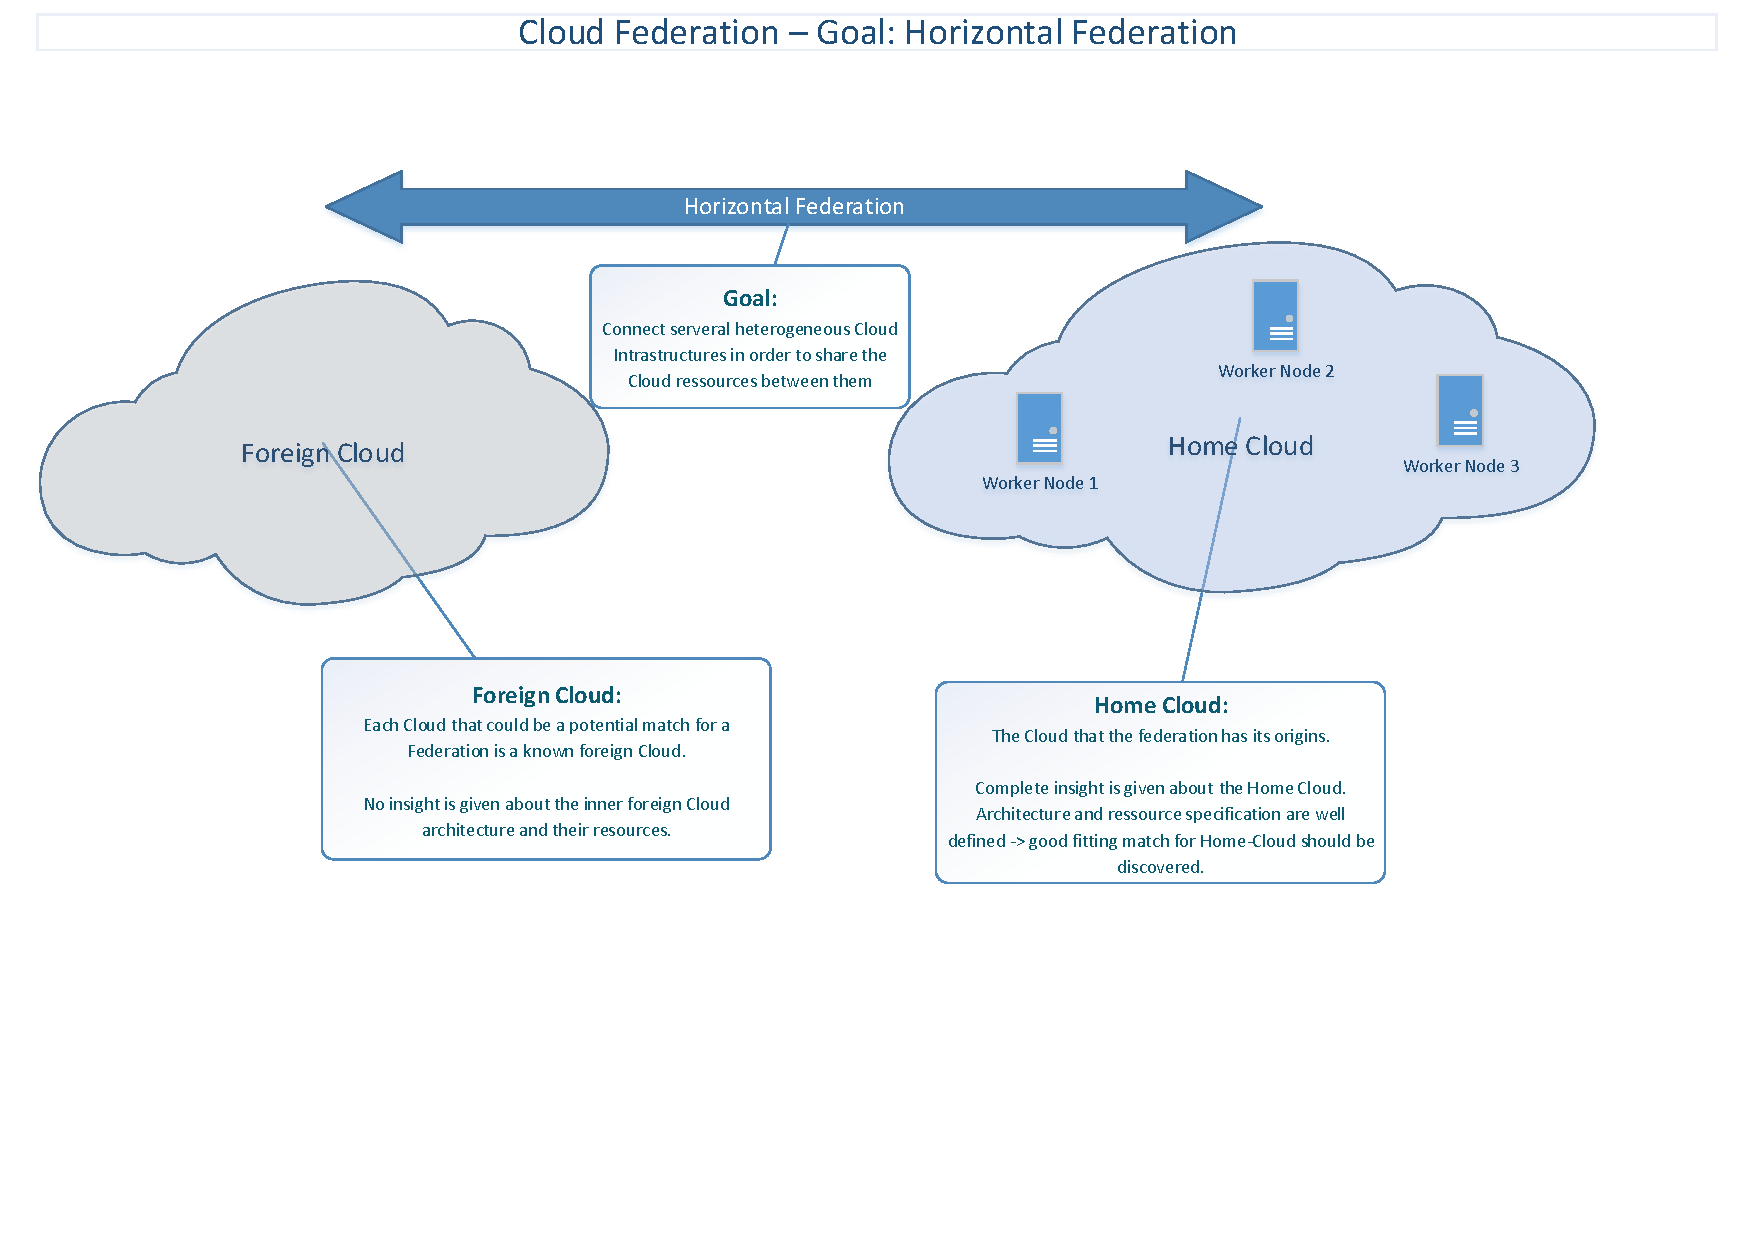
\includegraphics[width=0.8\textwidth]{./gfx/federationProposal.pdf}
 % 2014-05-19 - AgentFederation Proposal.pdf: 0x0 pixel, 300dpi, 0.00x0.00 cm, bb=
 \label{fig:federation_proposal}
\end{figure}

The Master thesis will have two different points of view in regards of Federation: Cloud- and Network-Federation. While the Cloud-Federation scenario is pointing out the high-level handling and cares about federation policies, the Network-Federation cares about the low-level network layers that needs to be connected somehow.

\newpage
\section{Cloud-Federation}
The Cloud-Federation part will have an Agent-oriented design in order to cope with different aspects in a Cloud-Federation scenario: Discovery of other Clouds, Policy and Resource handshaking and a security context establishment.

\begin{figure}[h!]
 \centering
 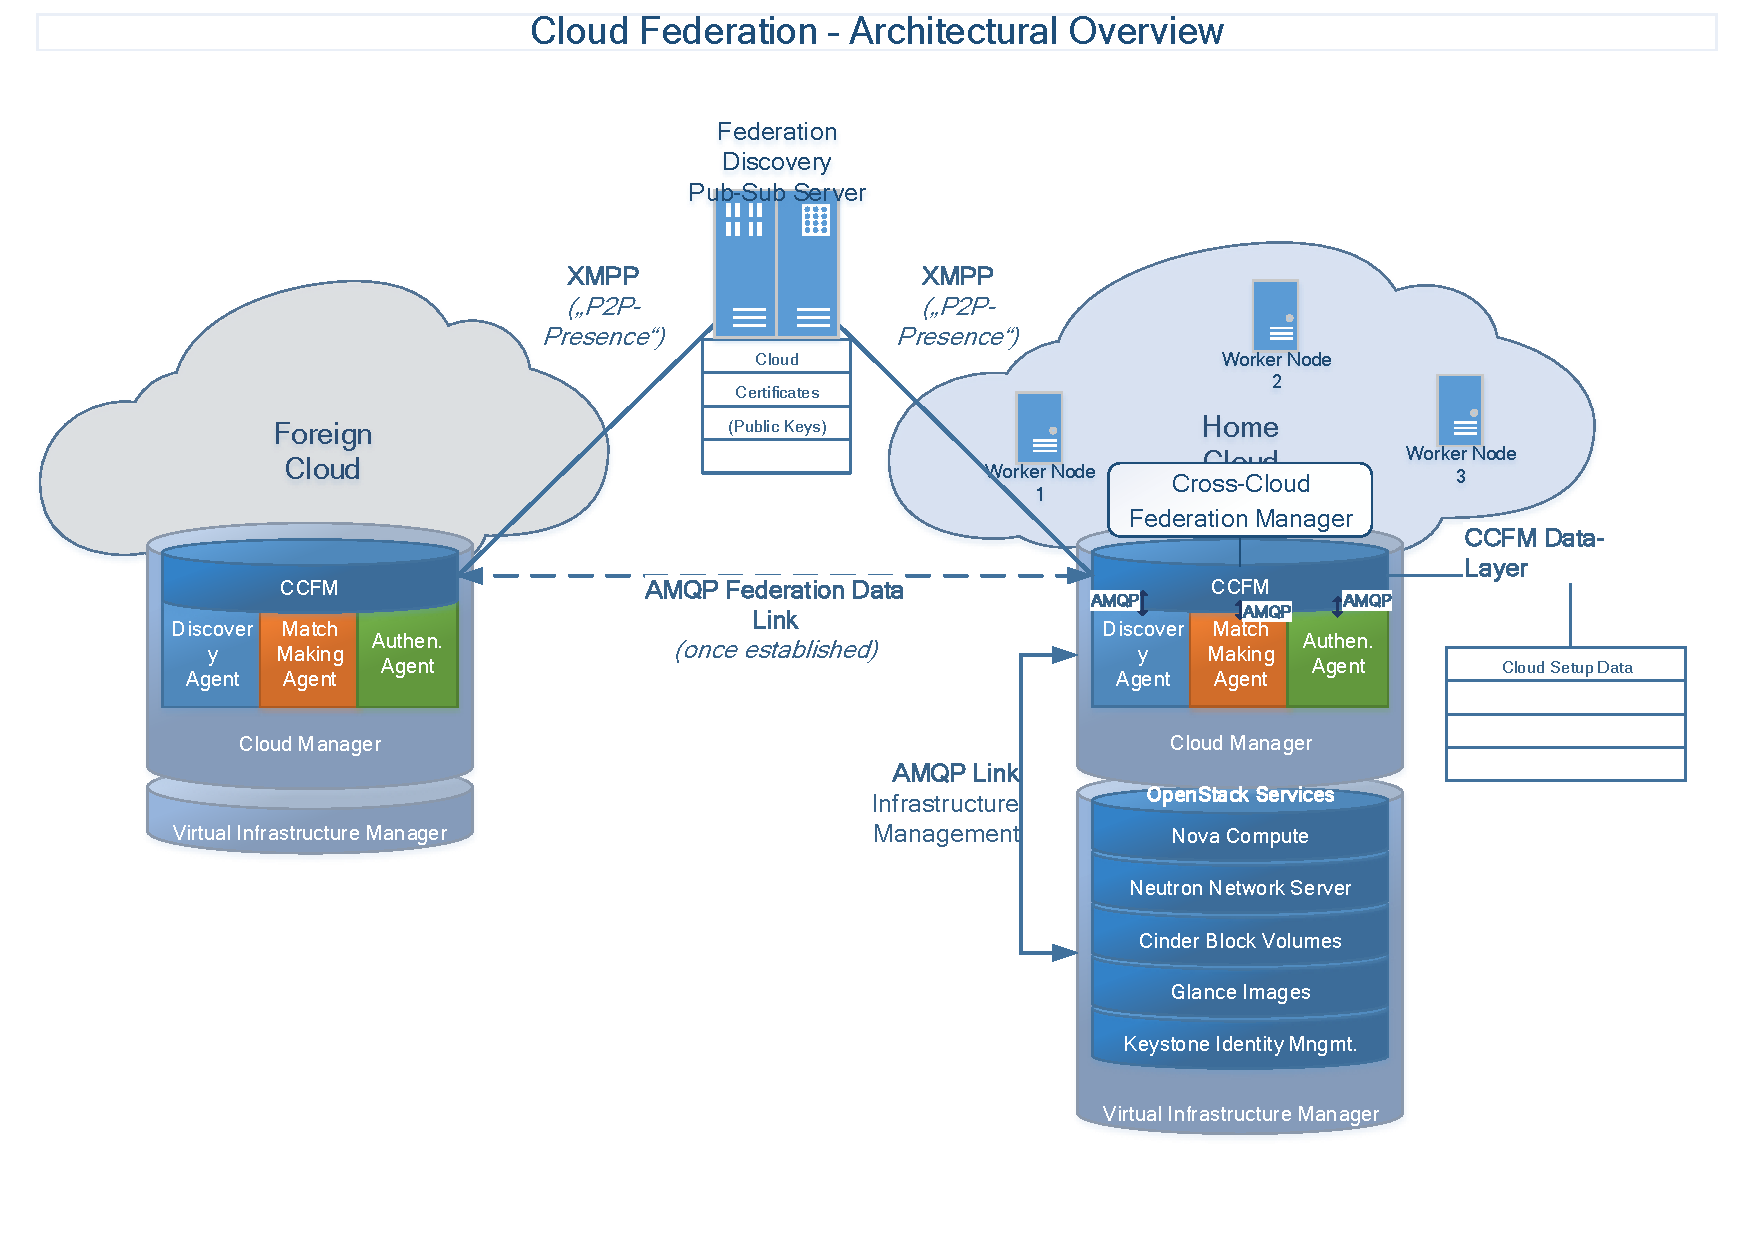
\includegraphics[width=0.8\textwidth]{./gfx/cloudFederation.pdf}
 % 2014-05-19 - AgentFederation Proposal.pdf: 0x0 pixel, 300dpi, 0.00x0.00 cm, bb=
 \label{fig:cloudFederation}
\end{figure}


\section{Network-Federation}
Network Federation cares about the federation connectivity of several OpenFlow driven Software Defined Networks. While the agent based Cloud-Federation is a vital aspect for the cloud management, the focus of this Master Thesis will be relying on the network Federation. A possible Network Federation, using OpenVirteX as an OpenFlow proxy could look, as described in figure \ref{fig:networkFederation}

\begin{figure}[h!]
 \centering
 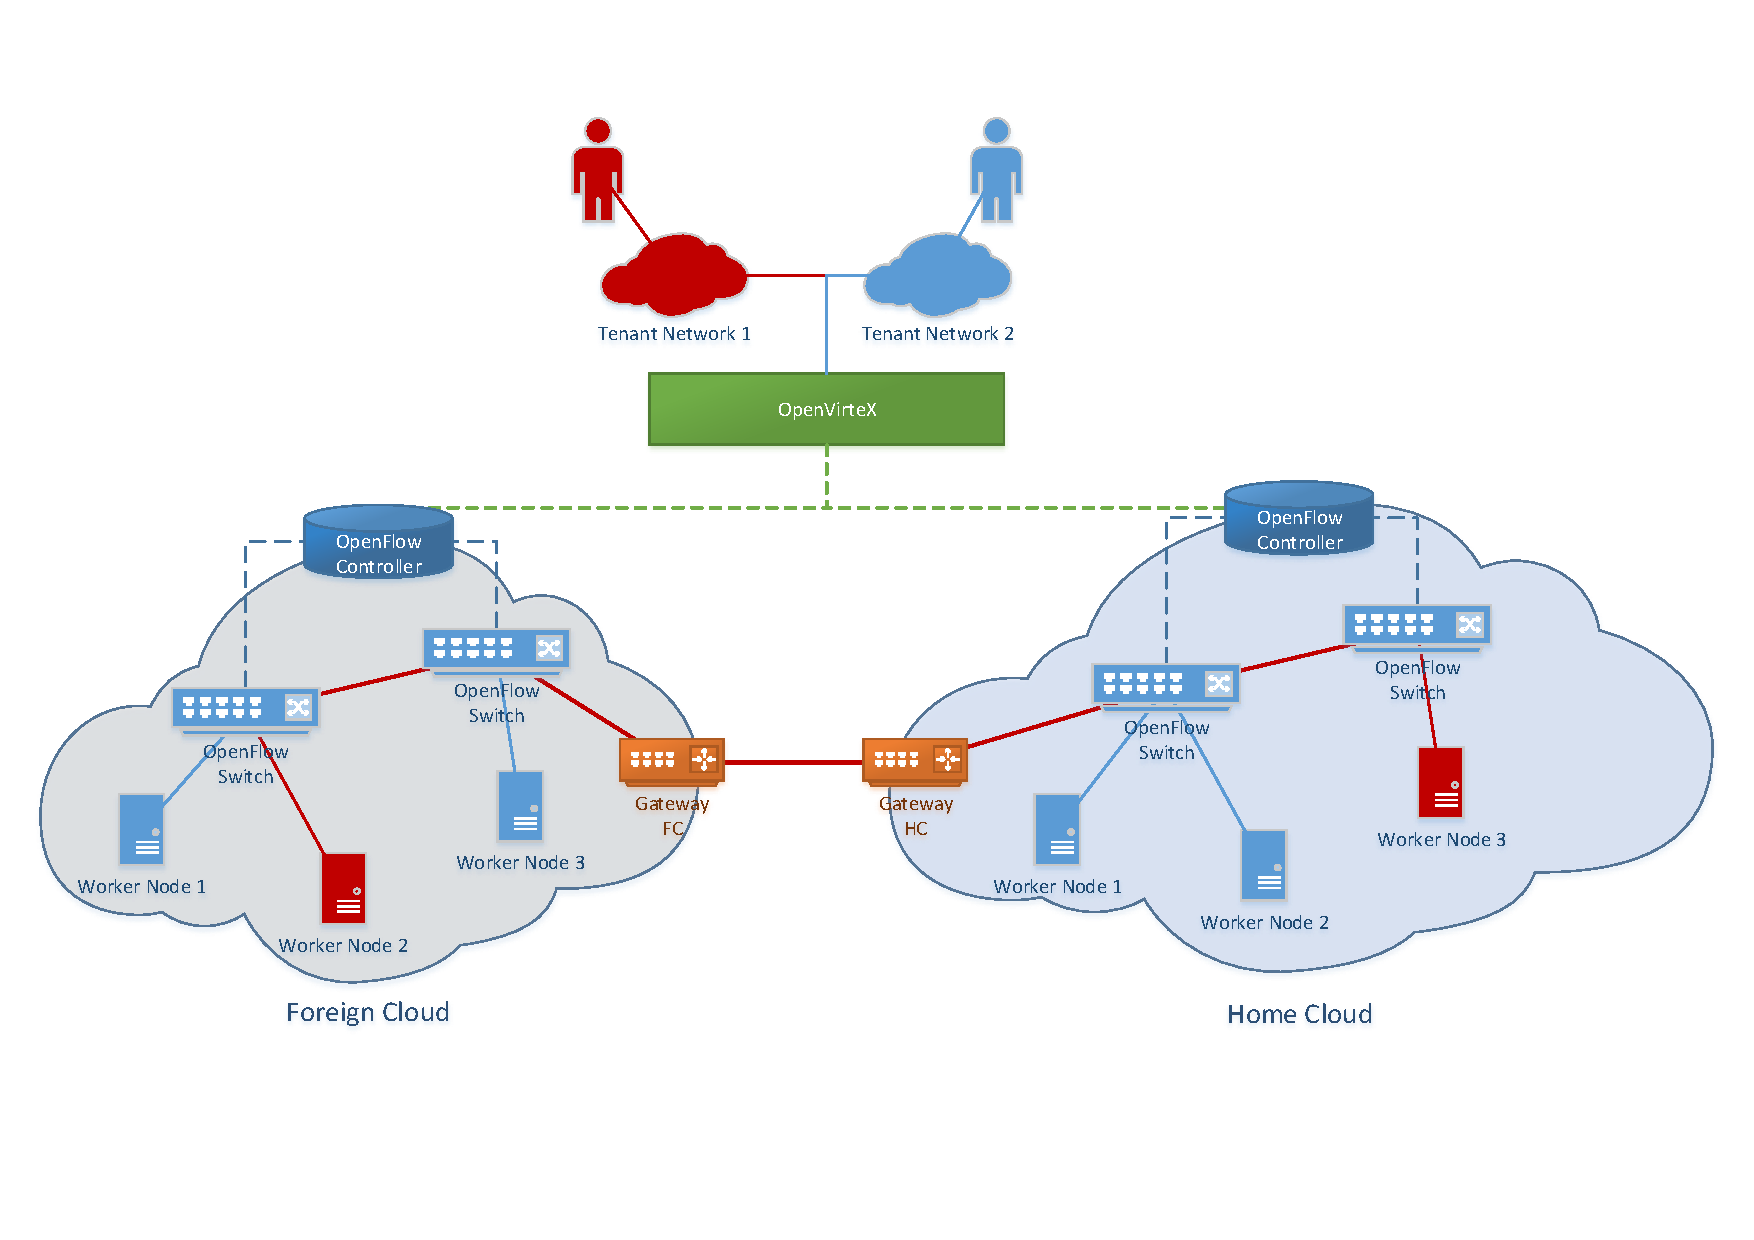
\includegraphics[width=0.8\textwidth]{./gfx/networkFederation.pdf}
 % 2014-05-19 - AgentFederation Proposal.pdf: 0x0 pixel, 300dpi, 0.00x0.00 cm, bb=
 \label{fig:federation_proposal}
\end{figure}


\newpage
\section{Research \& Development Tasks}
\begin{itemize}
	\item \textbf{Cloud Discovery} \\(Technical Implementation on an Agent based Platform)
	\item \textbf{Cloud Federation on the Data Level} \\(User- \& VM Image-Data, Theoretical Approach at first, could be made technical optionally)
	\item \textbf{Cloud Federation on the Network-Level} \\(Core Area, Technical Focus of Implementation as well as Theoretical discourse)
	\item \textit{\textbf{Cloud Federation Security - Authentication and Authorization}} \\(Will be approached on a Theoretical Level)
\end{itemize}

\section{Technologies of Interest}
\begin{itemize}
	\item{\textbf{Software Defined Networking:}}
	\begin{itemize}
		\item OpenFlow
		\item OpenVirteX (OpenFlow Proxy-Controller)
		\item Mininet (OpenFlow enabled SDN simulation)
		\item VirtualBox (As a Virtualization Hypervisor for Simulation purposes)
		\item OpenStack \& KVM (optional) (for a "real" Cloud environment setup)
		\item Python \& Java (as Mininet \& OpenVirteX are using these languages)
	\end{itemize}
	\item{\textbf{Agent based Cloud Federation:}}
	\begin{itemize}
		\item Scala + Akka (Java based language + Actor model for distributed, parallel tasks)
	\end{itemize}
\end{itemize}

\end{document}
